\documentclass[12pt,a4paper]{article}
\usepackage{inverba, apacite}

\newcommand{\userName}{Cullyn Newman} 
\newcommand{\class}{PHL 316U} 
\newcommand{\theTitle}{Argumentative Meta-Analysis of Contemporary Liberal Democracy and Freedom}
\setlength\headheight{20pt}
\setlength{\parindent}{0pt}
\title{\hypertarget{home}\theTitle\vspace*{-0.4cm}}
\author{\normalsize\userName}
\date{\vspace*{-0.5cm}\small\today}
\renewcommand{\baselinestretch}{1.618} 


\usepackage{pgfplots}
\begin{document}
\pgfplotsset{compat=newest}
 
 
\usepgfplotslibrary{patchplots}
%%%%%%%%%%%%%%%%%%%%%%%%%%%%%%%%%%%%%%%%%%%%%%%%%%%%%%%%%%%%%%%%%%%%%
\maketitle
\begin{abstract}
   \cite{neo}

   \cite{craft}

   \cite{direct}

   \cite{people}

   \cite{tom}

   
\end{abstract}
\newpage
\fancyhead{}
\fancyhead[R]{\hyperlink{home}{\nouppercase\leftmark}}
\fancyhead[L]{\theTitle}
\rhead{\hyperlink{home}{\thepage}}%%%%%%%%%%%%%%%%%%%%%%%%%%%%%%%%%%%%%%%%%%%%%%%%%%%%%%%%

\subsubsection{Introduction}
\vspace*{-12pt}
The main focus of this essay involves the views of both David Harvey and Richard Sennett in regards to the dynamic intereaction between contemporary liberal democracy and freedom of various scales. While the arguments of the such authors will gravitate toward the center of the discussion, the works of others will be included in order to help establish the constraints on the increasingly complex intereaction between governance and freedom. 

Overall, Harvey critiques are more broad, tackling the current state of neoliberalism and it's relation to freedom, while Sennett critiques have an more indirect relation, as his focus is on work and culture and their roles in the complex system we find ourselves in. There is much to be discussed, so in this essay I start with an initial meta-analysis of freedom, governance, and systems, which will be used as a means to generate a more nuanced discussion designed to allow for more significant argumentative claims to be made on what society ought to strive for. Ultimately, I argue both authors tend to imply aspects contemporary democracy need to change in order to promote greater degrees of genuine freedom. 

\subsubsection{Thinking in Systems}
\vspace*{-12pt}
The initial urge when analyzing the works of Harvey and Sennett is to jump directly into the struggle between neoliberalism and socialism their democratic impact on our freedom. This relationship between modes of governance stems from core disagreements mainly involving decentralization vs.\ centralization, free markets vs.\ regulation, and aristocracy vs.\ meritocracy, with of course other disagreements about maximization of profits, value of work, and more. 

Unfortunately, terms like democracy, socialism, and capitalism get thrown around far to often, resulting such words being crude representations of various disagreements; confusion about such words often are the most significant barriers to productive discussion. Therefore, before I dive into an analysis of work of Harvey and Sennett, I would first like to establish the importance of system thinking as a means to reduce unproductive confusion due to our tendency to overly compress complex relationships. 

A fundamental observation about how most people tend to think was made apparent to me this year by a \href{https://vitalik.ca/general/2020/11/08/concave.html}{{\color{B-Cold} blog post}} made by Vitalik Buterin, a computer scientist, involving the differences in worldviews generalized into either a concave or convex representations. Other posts by him, and the book, \textit{Thinking in Systems: a Primer}, by Donella H. Meadows and Diana Wright have pushed me towards the adoption of system-like thinking that will be heavily used by me in this analysis. To help illustrate, here is a brief summary of Vatalik's work:


\begin{figure}[h]

   \centering
   \caption*{{\color{neg}Convex} vs.\ {\color{liorange}Concave} Dispositions~\cite{vitalik}}
   \tikzset{every picture/.style={line width=0.75pt}}
   \scalebox{.8}{
   \begin{tikzpicture}[x=0.75pt,y=0.75pt,yscale=-1,xscale=1, color=darkText]  
      \draw  [color=neg,draw opacity=1 ][line width=1.5]  (32.11,108.37) .. controls (130.29,195.43) and (205.81,176.42) .. (258.67,51.33) ;
      \draw [line width=1.5]    (31.89,34.33) -- (31.89,186) ;
      \draw [shift={(31.89,30.33)}, rotate = 90] [line width=0.08]  [draw opacity=0] (13.4,-6.43) -- (0,0) -- (13.4,6.44) -- (8.9,0) -- cycle    ;
      \draw [line width=1.5]    (260.67,185) -- (31.89,185) ;
      \draw (31.89,194) node [anchor=north west][inner sep=0.75pt]   [align=left] {Option A};
      \draw (196,194) node [anchor=north west][inner sep=0.75pt]   [align=left] {Option B};
      \draw (110,194) node [anchor=north west][inner sep=0.75pt]   [align=left] {<< Policy >>};
      \draw (7,178) node [anchor=north west][inner sep=0.75pt]  [rotate=-270] [align=left] {Quality of Outcome};
   \end{tikzpicture}
      \hspace*{24pt}
   \begin{tikzpicture}[x=0.75pt,y=0.75pt,yscale=-1,xscale=1, color=darkText]
      \draw  [color=liorange, draw opacity=1 ][line width=1.5]  (576.4,166.63) ..controls (497.76,55.18) and (423.36,42.44) .. (353.2,128.4) ;
      \draw  [line width=1.5]    (352.89,37.33) -- (352.89,186) ;
      \draw [shift={(352.89,33.33)}, rotate = 90, color=darkText][line width=0.08] [draw opacity=0] (13.4,-6.43) -- (0,0) -- (13.4,6.44) -- (8.9,0) -- cycle    ;
      \draw [line width=1.5]    (577.67,185) -- (352.89,185) ;
      \draw (352.89,194) node [anchor=north west][inner sep=0.75pt]   [align=left]{Option A};
      \draw (517,194) node [anchor=north west][inner sep=0.75pt]   [align=left]{Option B};
      \draw (433,194) node [anchor=north west][inner sep=0.75pt]   [align=left] {<< Policy >>};
      \draw (320,178) node [anchor=north west][inner sep=0.75pt]  [rotate=-270][align=left] {Quality of Outcome};
   \end{tikzpicture}}
             
\end{figure}

Essentially what this is describing is the tendency to gravitate toward the idea that one of two options is correct (convex), or that a combination tends to yield the best result (concave). Ironically, this dichotomy itself raises a meta concave and convex analysis about each philosphy. Taking a meta-concave approach: both are useful and each can have a greater degree of usefulness in terms of making useful predictions. However, elaborating superiority of such views is not why I bring this up. As Vitalik describes,

\begin{quotation}
   \color{G-Moon}
   \noindent ``Convex and concave are terms best suited to mathematical functions where the input and the output are both one-dimensional. The real world is high-dimensional---and as machine-learning researchers have now well established, in high-dimensional environments the most common setting that you can expect to find yourself in is not a universally convex or universally concave one, but rather a saddle point''~\cite{vitalik}
\end{quotation}

\begin{figure}[h]
   \centering
   \caption*{Graphical Representation of a Saddle Point}
   \scalebox{.8}{
   \begin{tikzpicture}
      \begin{axis}
         \addplot3 [surf, draw=black,domain=-1.2:1.2,domain y=-1.5:1.5,opacity=0.6] {x^2-y^2};
      \end{axis}
   \end{tikzpicture}}
\end{figure}

As you add more dimensions, then the complex intereaction between multiple concave and convex relationships produces local minima and maxima in the form of saddle points. Even with just three dimensions, one can see how compressing such views into one dimensional left of right thinking can result in demonstrability false predictions of quality of outcome. What happens when we take the on many multi-dimensional political philsophies? Exponential increases in compression difficulty of the diverse idea-spaces---something our minds certainly not well are equipped to handle. This is where system-thinking comes into play,

\begin{quotation}
   \color{G-Moon}
   \noindent``There are no separate systems. The world is a continuum. Where to draw a boundary around a system depends on the purpose of the discussion. We can't impose our will on a system. We can listen to what the system tells us, and discover how its properties and our values can work together to bring forth something much better than could ever be produced by our will alone.''~\cite{systems}
\end{quotation}

``Where we draw the boarders'' is the compression---we have to be careful when doing this as it's very easy to draw wrong conclusions, but vital, because we can't see the system as a whole. Listening involes the investgation and careful drawing of boarders around local systems we can observe. This is a tremendous distinction that needs to be constantly reinforced since we suffer from multitude of cognitive biases that interfere with our own relative views of reality, which act to increase the probability of poor compressions.


\subsubsection{The Complexity of Freedom}
\vspace*{-12pt}


\newpage
\textbf{Counter-arguments}

\textbf{Rebuttals}

\textbf{Conclusion}




\clearpage
\bibliographystyle{apacite}
\bibliography{citations.bib}
%\endgroup
\end{document}